% declarar nenhum cabeçalho

\section{Transporte}
\subsection{Voltar para casa}

Para os calouros de fora de Campinas, além de escolher a nova morada é
importante recolher informações sobre como realizar o trajeto entre sua cidade e
Campinas.

A forma usual é ir de ônibus, mas tenha em mente que a rodoviária é longe e os
trajetos de ônibus até lá são demorados. O endereço da rodoviária é Rua Barão de
Parnaíba, 690. Há duas linhas que passam por lá: o 3.32 (que passa dentro da
Unicamp) para dentro da rodoviária, mas demora mais pra chegar que o 3.31, que
sai do terminal e para do lado de fora da rodoviária. Em horários de pico, o
trajeto pode demorar quase uma hora, então cuidado para não perder o horário do
ônibus para sua cidade.

Os que vêm de mais longe certamente farão uso do aeroporto de Viracopos, cujo
telefone é 3725-5000. Para chegar ao aeroporto existe a linha 1.93 que sai da
rodoviária e vai para o aeroporto, e também faz o trajeto de volta. Porém ir com
ônibus circular pode ser um transtorno quando estiver com mala grande. Uma outra
alternativa é a Caprioli que também faz o trajeto da rodoviária para o
aeroporto. A passagem da Caprioli custa em torno de R\$8,00 e os horários podem
ser conferidos no site \url{caprioli.com.br}.

Para quem for usar os aeroportos da Grande São Paulo (Congonhas e Guarulhos),
também existe o translado da Caprioli. A tarifa sai em torno de R\$30,00 a
R\$35,00 e os horários podem ser conferidos no site da Caprioli.

\subsubsection*{Caronas}

Uma forma barata e divertida de viajar, além de minimizar o tempo e dinheiro
gastos na viagem, é juntando alguns estudantes no mesmo carro e dividir as
despesas.
\begin{figure}[h!]
    \centering
    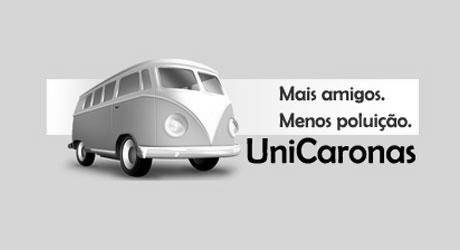
\includegraphics[width=.45\textwidth]{img/barao/unicaronas.jpg}
\end{figure}

O site UniCaronas (\url{unicaronas.com.br}) foi desenvolvido por dois
engenheiros de computação da Unicamp, com o intuito de facilitar o deslocamento
dos alunos entre cidades. Criado em 2007 como Caronas Unicamp e disponível 
apenas para alunos da Unicamp, atualmente o site possui mais de 20 mil usuários 
e media carona entre alunos de diversas universidades para várias cidades de 
vários estados, mas novas cidades podem ser inseridas à medida que aumentar a 
demanda por elas. No entanto, o site serve apenas para colocar os motoristas e 
caronistas em contato, não assumindo responsabilidades sobre nenhuma das partes.

\subsection{Carro}

Para aqueles que tenham seu próprio veículo, é bom saber que a Unicamp tem
poucas vagas próximas aos locais de aulas. E o número de fiscais de trânsito tem
aumentado muito dentro do Campus.

\subsubsection*{Autoescolas}

Se você ainda não tem CNH e pretende obtê-la em Campinas, existem três opções de
autoescola em Barão Geraldo:

\begin{itemize}
    \item  \textbf{Auto Escola Avenida}
        \\Endereço: Av. Albino J. B. De Oliveira, 658
        \\Telefone: (19) 3288-0588

    \item  \textbf{Auto Escola Advanced}
        \\Endereço: Av. Santa Isabel, 80
        \\Telefone: (19) 3289-9499

    \item  \textbf{Auto Escola Mario Trentin}
        \\Endereço: Av. Santa Isabel, 513
        \\Telefone: (19) 3388-0513 / (19) 3289-2614
\end{itemize}

\subsubsection*{Recorrer de Multas}

Documentos:
\begin{itemize}
    \item  Notificação e Fotocopia.
    \item  CNH e Fotocopia.
    \item  Documento do Carro e Fotocopia.
    \item  Formulário: \url{www.emdec.com.br/eficiente/repositorio/EMDEC_documentos/5079.pdf}.
    \item  e anexos, se desejar.
\end{itemize}

E levá-los a:
\begin{itemize}
    \item   \textbf{EMDEC}
        \\Horário: De segunda a sexta-feira, das 8h as 17h.
        \\Endereço: Rua Dr. Salles Oliveira, 1028 -- Vila Industrial -- CEP 13035-270.
    \item   \textbf{Poupatempo (Centro)}
        \\Horário: Das 8h às 18h, de segunda a sexta-feira; e aos sábados, das 7h às 13h.
        \\Endereço: Av. Francisco Glicério, 935.
    \item   \textbf{Poupatempo (Campinas Shopping)}
        \\Horário: Das 9h às 19h, de segunda a sexta-feira; e aos sábados, das 8h às 14h.
        \\Endereço: Rua Jacy Teixeira de Camargo, 940.
\end{itemize}

Fonte: \url{www.emdec.com.br/eficiente/sites/portalemdec/pt-br/site.php?secao=multas&pub=31}

\subsection{Ciclovias e ciclofaixas}

Campinas possui cerca de 27 quilômetros de ciclovias e de ciclofaixas. Algumas dessas vias para 
bicicletas estão no distrito de Barão Geraldo. Uma delas é a ciclovia que liga o campus da Unicamp 
a Av. Albino J. B. de Oliveira. A outra é a ciclofaixa que liga a Av. Albino J. B. de Oliveira 
à moradia (Av. Santa Isabel).

Nos domingos e feriados, das 7 até as 12 horas, as ciclofaixas ficam abertas para os ciclistas.

\subsection{Ônibus}

Se não tem condução própria, ou carona, pode utilizar o transporte coletivo de
Campinas.

\begin{figure}[h!]
    \centering
    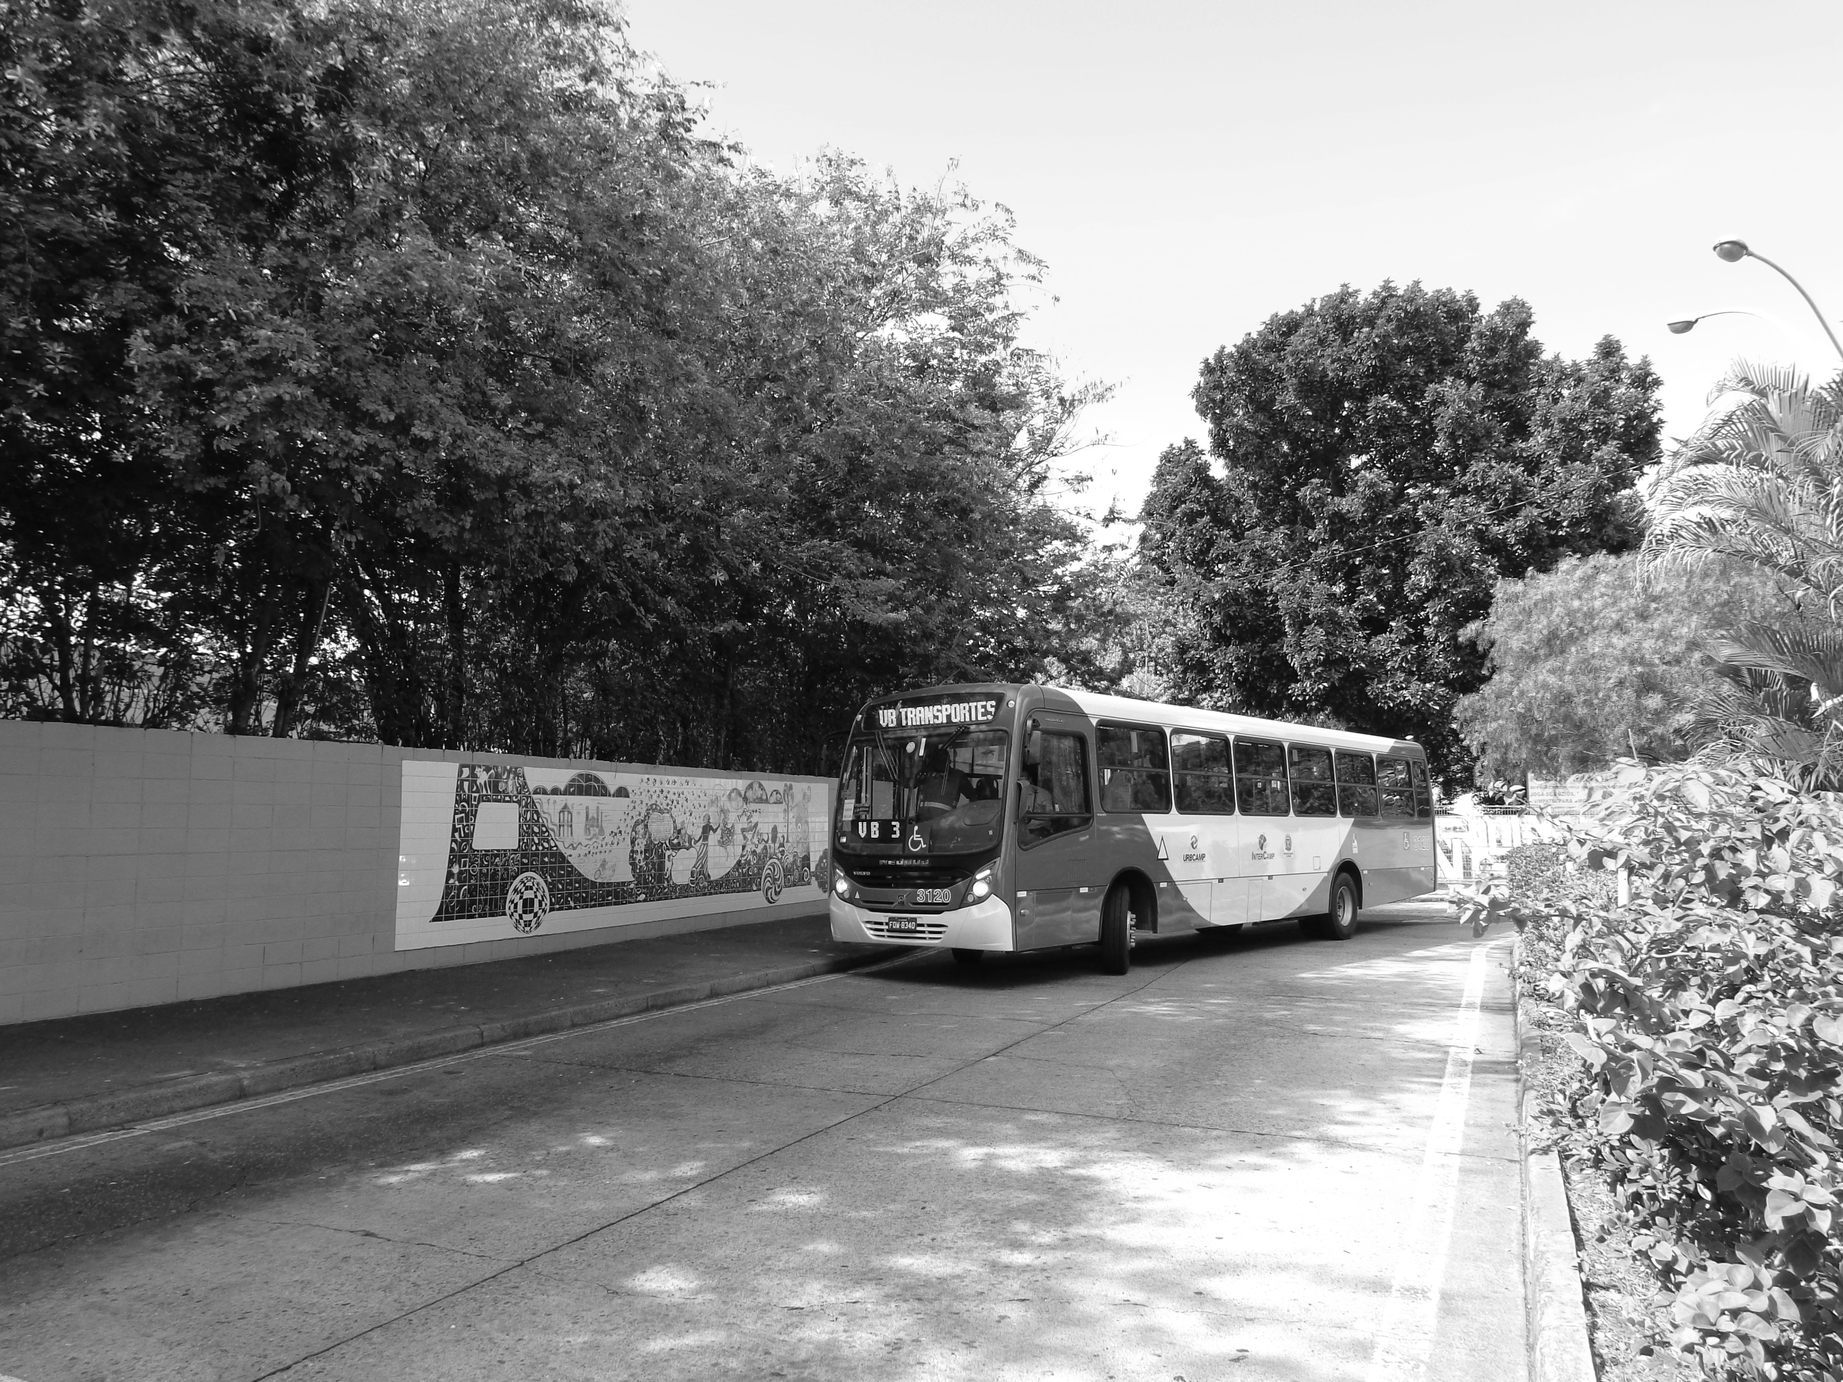
\includegraphics[width=.45\textwidth]{img/barao/onibus.jpg}
\end{figure}

Os ônibus em Campinas são identificados por um número de três dígitos, uma cor
(azul claro, azul escuro, vermelho ou verde), uma figura geométrica (círculo,
quadrado, triângulo ou tetragrama, para que os portadores de daltonismo possam
identificar os ônibus) e um nome. A tarifa (uma das mais caras do Brasil) foi
reajustada em junho de 2013 e é R\$3,00. Apesar de existir passe de estudante,
universitários não têm direito ao desconto, apenas estudantes de ensino
fundamental e médio.

Desde o começo de 2013, no último domingo de cada mês, os usuários do transporte 
público de Campinas podem usar os ônibus pagando metade da tarifa (o que dá R\$ 1,50). 
É o passe lazer. O benefício não está disponível para quem tem o VT (vale transporte).

Existe quatorze linhas de ônibus que ligam o centro, alguns distritos, bairros e
terminais de Campinas ao distrito de Barão Geraldo. Algumas linhas desembarcam
os passageiros no terminal de Barão Geraldo, de onde seguem em outros ônibus
para a universidade. Já outras linhas vão direto para o campus. As trocas de
ônibus dentro do Terminal de Barão Geraldo são gratuitas, o que não ocorre em
outros terminais (no Terminal Mercado, por exemplo).

Em 2008 foi construída a nova e moderna rodoviária de Campinas, o terminal
multimodal Ramos de Azevedo. Além de transporte interestadual e municipal, o
espaço agrega um terminal metropolitano com o intuito de ligar as cidades da
Região Metropilitana de Campinas. Algumas linhas de ônibus internos de Campinas
também passam neste Terminal, como a linha 3.32.

Veja as linhas de ônibus disponíveis abaixo:

\begin{itemize}
    \item  \textbf{1.34 -- Terminal Barão Geraldo (Inclusivo):} Sai do terminal
        do Ouro Verde, passa próximo ao Shopping Unimart, às avenidas Luís
        Smânio, Brasil, Theodureto de Almeida Camargo, Albino José Barbosa de
        Oliveira e vai para o terminal de Barão.

    \item  \textbf{2.10 -- Terminal Campo Grande / Shop. Dom Pedro / Terminal
        Barão Geraldo:} Sai do Terminal Campo Grande, passa pelo Shopping Dom
        Pedro, Terminal Barão Geraldo, avenida 1, rua Roxo Moreira (em frente à
        Reitoria), de novo pelo Shopping Dom Pedro, voltando para o Terminal
        Campo Grande.  Saindo do terminal de Barão, essa linha passa na rua Roxo
        Moreira e próximo à area de biológicas e da saúde (Hospital das Clínicas
        e Faculdade de Ciências Médicas). Passa apenas na região da reitoria e
        hospital.

    \item  \textbf{2.66 -- Terminal Padre Anchieta / Hospital das Clínicas:} Sai
        do Terminal Padre Anchieta, passa pelo Makro, Shopping e rodovia D.
        Pedro, em frente ao Terminal Barão Geraldo (mas não entra), avenida 2,
        Unicamp, PUC, Rodovia D. Pedro I voltando para o Terminal Padre
        Anchieta.

    \item  \textbf{2.69 -- Terminal Padre Anchieta / Terminal Barão Geraldo:}
        Assim como o 2.66, sai do Terminal Padre Anchieta, mas faz um trajeto
        diferente do 2.66, indo até o terminal de Barão. O intervalo entre os
        ônibus é de 90 minutos em dias úteis, e de 100 minutos nos sábados,
        domingos e feriados.

    \item  \textbf{3.00 -- Sousas / Terminal Barão Geraldo:} Sai de Sousas (um
        dos distritos de Campinas, assim como Barão Geraldo), passa pelo
        Shopping Galleria, pelo terminal do Shopping Dom Pedro, rodovias Heitor
        Penteado e Dom Pedro, tapetão e vai em direção ao terminal de Barão
        Geraldo.  O problema é que o intervalo entre os ônibus é de 45 minutos.

    \item  \textbf{3.21 -- Centro Médico/Bosque das Palmeiras:} Sai do Terminal
        Barão e leva à Cidade Universitária II, passando pela avenida 2 e em
        frente ao Centro Médico.

    \item  \textbf{3.28 -- Guará:} Assim como o 3.21 leva à Cidade Universitária
        II, mas vai pela estrada da Rhodia até a Cidade Universitária e segue
        até o Guará.

    \item  \textbf{3.29 -- Terminal Barão Geraldo / Cidade Judiciária:} Sai do
        terminal de Barão, passa pela avenida 2, pela Unicamp, por algumas ruas
        e avenidas do bairro fazenda Santa Cândida e vai até a estação da Cidade
        Judiciária. O intervalo entre ônibus pode variar de 27 a 40 minutos nos
        dias úteis, e é de 40 minutos aos sábados, domingos e feriados.

    \item  \textbf{3.30 -- Unicamp / Hospital das Clínicas:} Do Terminal Central
        de Campinas à Unicamp, passando pela rótula e avenidas Moraes Salles,
        Orosimbo Maia, Anchieta (prefeitura), Brasil e tapetão. Funciona das 6
        às 19h30, a cada 15 minutos em média (depende do horário), de segunda a
        sexta-feira (não funciona nos sábados, domingos e feriados). Para ir do
        centro até a Unicamp e da Unicamp até o centro, essa linha é mais rápida
        que o 3.32, só que quase sempre os ônibus dessa linha estão cheios.

    \item  \textbf{3.31 -- Terminal Barão Geraldo / Rodoviária:} Sai do terminal
        Barão Geraldo e passa na rodoviária. É a opção mais rápida saindo de
        Barão, levando cerca de 30 min (sem trânsito) em comparação com os mais
        de 40 minutos do 3.32. Passa também pelo Cambuí.

    \item  \textbf{3.32 -- Terminal Barão Geraldo / Hospital das Clínicas /
        Rodoviária (Inclusivo):} Do Terminal Metropolitano até a Unicamp e
        depois para o terminal Barão Geraldo, passando pela rótula, pela
        rodoviária nova e pelas avenidas Campos Sales, Anchieta (prefeitura),
        Orozimbo Maia, Brasil, Theodureto de Almeida Camargo e outras. Funciona
        das 6 às 23 horas, a cada 15 minutos em média, todos os dias. Essa linha
        vai diretamente para a Unicamp, porém demora muito para ir do terminal
        metropolitano/centro até a Unicamp e da Unicamp até o centro/terminal
        metropolitano e quase sempre os ônibus dessa linha estão muito cheios,
        apesar de que, ao chegar ou sair da Unicamp eles estão com poucos
        passageiros. No sentido terminal de Barão Geraldo -- terminal
        metropolitano, esse ônibus para no ponto localizado ao lado do IC-1.

    \item  \textbf{3.33 -- Terminal Barão Geraldo / Circular Rótula:} Do
        Terminal Barão Geraldo ao centro de Campinas, passando pela rótula,
        Orosimbo Maia, Anchieta (prefeitura) e pelo Terminal Central. Não passa
        pela Unicamp, então para chegar à Unicamp, deve pegar a linha 3.29, 3.32
        ou 3.37. Funciona das 5h30 às 23h30, a cada 10 minutos, todos os dias.

    \item  \textbf{3.37 -- Hospital das Clínicas:} Antiga linha 3.87. Do 
        Terminal Barão Geraldo ao HC, passando pela Unicamp. Funciona das 
        5h30 às 23h30, a cada 15 minutos, de segunda a sexta-feira. Passa 
        pelo IC aos domingos.

    \item  \textbf{3.38 -- Terminal Barão Geraldo / Shopping D. Pedro / Shopping
        Iguatemi:} Linha que passa pelos dois principais shoppings da cidade.
        Funciona das 5:50 às 23:15, de segunda à sábado, a cada 30 minutos e em
        domingos e feriados funciona das 9:00 às 21:40, a cada 40 minutos.
\end{itemize}

E se pintar qualquer dúvida é só entrar no site da EMDEC
(\url{www.emdec.com.br}) ou da TRANSURC (\url{transurc.com.br}) para ver os
horários e a trajetória de todas as linhas de Campinas.

\subsubsection*{Bilhete Único}

O bilhete único foi implantado com o objetivo de facilitar o transporte daqueles
que se utilizam de ônibus. No prazo de 2 horas, o usuário pode usar até três ônibus 
pagando apenas uma passagem. Para quem usa mais de três ônibus e quer aumentar o 
número de integrações, tem de ir à sede da TRANSURC, localizado na rua Onze de Agosto, 
757, Centro. O bilhete único também vale para o passe lazer.

Para adquiri-lo, dirija-se ao Terminal Barão Geraldo, Central, Ouro Verde, Campo
Grande ou Mercado, munido de seu RG e CPF. Você preencherá um cadastro e
retornará após alguns dias para retirar seu cartão. Para a primeira recarga,
exige-se o pagamento de duas tarifas (o que atualmente fica em R\$ 6,00).

Para recarregar o cartão, além dos terminais, também tem diversos
estabelecimentos comerciais credenciados a fazer a recarga do cartão, que podem
ser vistos na página: \url{transurc.com.br/site/?page_id=31}.
